\documentclass[a4paper]{report}
\usepackage{a4wide}
\usepackage[utf8]{inputenc}
\usepackage{parskip}
\usepackage{hyperref}
\usepackage{epsfig}
\usepackage{background}
\usepackage{mathptmx}

% To avoid tikz error, see https://tex.stackexchange.com/questions/165929/semiverbatim-with-tikz-in-beamer
\makeatletter
\global\let\tikz@ensure@dollar@catcode=\relax
\makeatother

\backgroundsetup{
scale=1,
angle=0,
opacity=1,
contents={
\includegraphics[width=\paperwidth,height=\paperheight]{images/spi-front.jpg}}
}

\hypersetup{
  colorlinks   = true,
  urlcolor     = blue,
  linkcolor    = blue,
  pdfinfo = {
    Title = {SPI Annual Report 2019},
    Author = {Software in the Public Interest, Inc.},
    Keywords = {SPI, free software, open source, FOSS, annual report, charity, non-profit, 501c3},
  }
}

\begin{document}

\title{Software in the Public Interest, Inc.\\
2019 Annual Report}
\date{XXXX XX, 2019}

\maketitle

\newpage

\backgroundsetup{
scale=1,
angle=0,
opacity=1,
contents={
\includegraphics[width=\paperwidth,height=\paperheight]{images/spi-content.jpg}}
}

\hspace{1em}

To the membership, board and friends of Software in the Public Interest, Inc:

As mandated by Article 8 of the SPI Bylaws, I respectfully submit this annual
report on the activities of Software in the Public Interest, Inc. and extend my
thanks to all of those who contributed to the mission of SPI in the past year.

  \emph{-- Michael Schultheiss, SPI President}

\newpage

\tableofcontents

\newpage

\chapter{President's Welcome}
\label{sec:president}

The mission of SPI is to help substantial and significant open source
projects by handling their non-technical administrative tasks so that
they aren't required to operate their own legal entity.

During the current board term, SPI (its officers, directors, contractors
and volunteers) has continued to refine and improve its processes and
response time.  Treasury sprints prior to in-person board meetings
continue to be highly productive and I strongly recommend they continue
going forward when in person meetings are again practical. SPI Vice
President Stephen Frost has been instrumental in refining our
contracting process and has been an excellent liaison with SPI's legal
counsel.

SPI continues to fill a needed role in the free and open source software
community. Sister organizations exist and are not competitors for
hosting projects but have differing roles in the ecosystem. We welcome
associated projects to freely move to other umbrella organizations if
they need more than SPI's relatively hands off manner can provide as
well as welcome any projects who prefer to join SPI due to our focus.

SPI had its financial statements independently audited for the 2018
calendar year and plans to continue having its financial statements
independently audited annually going forward.

The SPI board is extremely thankful for the work Martin Michlmayr has
done working with SPI's auditor and streamlining our bookkeeping. Martin
has been instrumental in releasing periodic treasury reports, updating
the financial toolset and assisting the treasury team with data
validation.

Thank you again to all SPI officers, directors, contractors, volunteers
and members. SPI continues to thrive thanks to your contributions.

  \emph{-- Michael Schultheiss, SPI President}

\chapter{Committee Reports}
\section{Membership Committee}

\subsection{Statistics}

On January 1, 2019 we had 212 contributing and 1082 non-contributing
members.  On December 31, 2019 there were 222 contributing members and
1138 non-contributing members.  This is an increase of 10 contributing
members and an increase of 56 non-contributing members.

\chapter{Board Report}
\section{Board Members}

Board members as of January 1, 2019:

\begin{itemize}
\item Jimmy Kaplowitz (President)
\item Luca Filipozzi (Vice President)
\item Tim Potter (Secretary)
\item Michael Schultheiss (Treasurer)
\item Stephen Frost
\item Dimitri John Ledkov
\item Martin Michlmayr
\item Andrew Tridgell
\item Martin Zobel-Helas
\end{itemize}

Board members as of December 31, 2019:

\begin{itemize}
\item Michael Schultheiss (President)
\item Stephen Frost (Vice President)
\item Tim Potter (Secretary)
\item Martin Zobel-Helas (Treasurer)
\item Luca Filipozzi
\item Forrest Fleming
\item Chris Lamb
\item Héctor Orón Martínez
\item Andrew Tridgell
\end{itemize}

Advisors to the board as of December 31, 2019:

\begin{itemize}
\item Software Freedom Law Center (SFLC), legal counsel
\item Sam Hartman, Debian Project representative
\item Robert Treat, PostgreSQL Project representative
\end{itemize}

\section{Board Changes}

Changes that occurred during the year:

\begin{itemize}

\item Martin Michlmayr resigned from the board in March 2019.
We'd like to thank Martin for his contributions!

\item The board appointed Renee Phillips as an interim director in
April 2019.

\item The terms for Dimitri John Ledkov, Jimmy Kaplowitz, Renee Phillips
and Martin Zobel-Helas expired in July 2019.  Martin sought, and
obtained, re-election.  We'd like to thank Dimitri John Ledkov, Jimmy
Kaplowitz and Renee Phillips for their work on the board.  Forrest
Fleming, Chris Lamb and Héctor Orón Martínez joined the board as part
of the same election.

\item On August 12, 2019 the board voted to appoint the following
officers:

\begin{itemize}
\item President: Michael Schultheiss
\item Vice President: Stephen Frost
\item Secretary: Tim Potter
\item Treasurer: Martin Zobel-Helas
\end{itemize}

\end{itemize}

\section{Elections}

A board membership election was conducted in July 2019.  There were 4
board seats up for election.  Nominations were received from Forrest
Fleming, Chris Lamb, Héctor Orón Martínez and Martin Zobel-Helas.  Since
there were 4 nominations for 4 board seats, no vote was required and all
four candidates were elected for a 3 year term.

\section{Face-to-face Meetings}

The SPI board held two face-to-face meetings in 2019.

At the end of February and the beginning of March, a treasurer sprint
was held for two days, followed by a two-day board meeting.  Meeting
space was kindly provided by the Fintech Open Source Foundation
FINOS) and Crunchy Data.

During the treasurer sprint, the team worked on closing the books
for 2018.  There was also discussion about improving the processes
and workflows and creation more documentation.

During the board meeting, topics such as IT, contractors, budgets
and the intake process were discussed.

The board held another meeting in November 2019 with the newly
elected board.  Meeting space was provided by Hudson River Trading
in New York.  The board discussed the results from the first external
audit, contractors, policies and documentation, infrastructure,
and other topics.  During a preceding treasurer sprint, outstanding
payment requests were worked on.

\begin{figure*}[h]
\centering

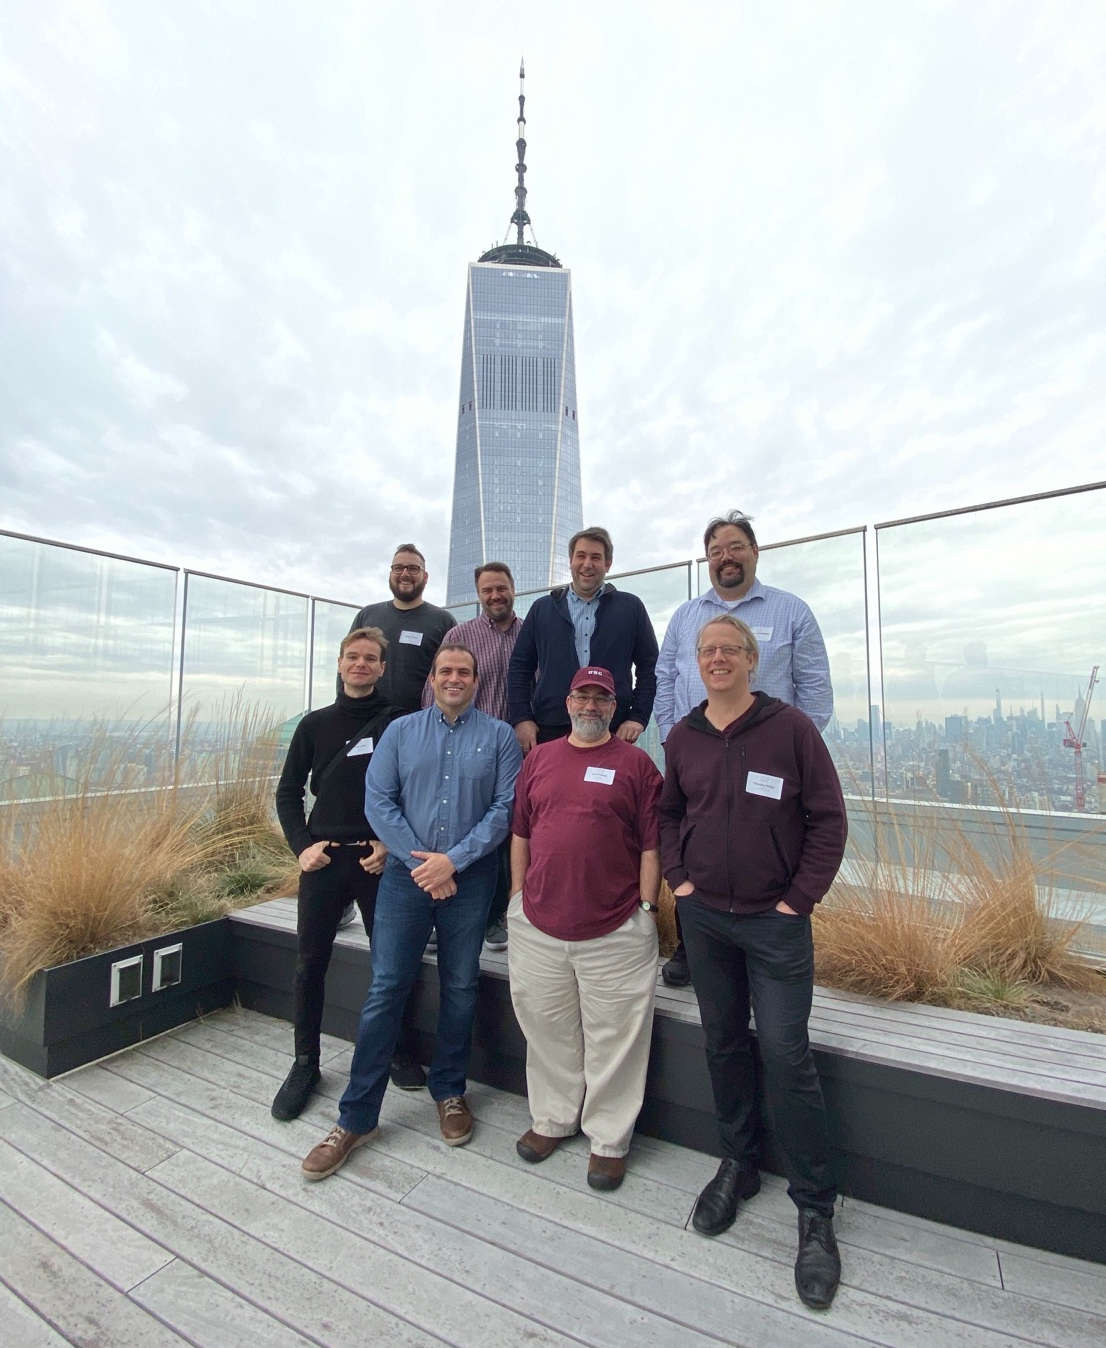
\includegraphics[scale=1.25]{images/2019-november-f2f}

\caption{Face-to-face meeting in New York (November 2019). Front (left
to right): Chris Lamb, Héctor Orón Martínez, Luca Filipozzi, and Tim
Potter.  Back: Forrest Fleming, Stephen Frost, Martin Zobel-Helas,
and Michael Schultheiss}

\end{figure*}

\chapter{Treasury Report}

This report uses a cash-based method of accounting, recording donations
when deposited (not when the check was written or received by us) and
recording expenses when sent or scheduled for payment (not when
incurred).

{\em These figures are provisional and subject to change.}

\section{Income Statement}

This covers the Period January 1, 2019 -- December 31, 2019

\begin{verbatim}
FIXME
\end{verbatim}

\section{Balance Sheet}

\begin{verbatim}
Balance Sheet as of December 31, 2019

FIXME
\end{verbatim}

\chapter{Member Project Reports}

\section{New Associated Projects}

\subsection{Arch Linux 32}

Archlinux32 is a community maintained fork of the Arch Linux
distribution for Intel 32-bit (IA-32) type of CPUs (similar of what
ArchlinuxARM is doing for ARM-based CPUs).

The official support for Intel 32-bit (IA32) has been dropped as of
November 2017.  Archlinux32 plays the catch-up game with upstream Arch
Linux to still provide a usable 32-bit version of Arch Linux.

Archlinux32 has a sophisticated build system keeping track of all
dependencies between packages.  This is especially challenging as
important packages can stop building any time and people expect packages
to be on the bleeding edge (the very purpose of Arch Linux).

\subsection{OpenSAF}

OpenSAF is an open source community with projects focused on high
availability (HA) middleware.  The goal of OpenSAF projects is to
develop HA middleware that is consistent with the Service Availability
Forum (SA Forum) specifications.

\subsection{Translatewiki.net}

Translatewiki.net is a translation community and a localization platform
for free and open source projects. Our mission is to streamline the
management of software interface translations, so that FOSS projects,
both small and large, are accessible to people around the world, in a
language they prefer to use. For FOSS projects, we provide a turn-key
solution for getting their software translated in hundreds of languages
and advice on software internationalization. For volunteer translators,
we provide a unified process to translate many FOSS projects ---  no
need to request permissions, email files or work with version control
systems.

\section{Projects No Longer Associated with SPI}

\begin{itemize}

\item Drizzle was fork of the MySQL project originally made in 2008.
The project has been defunct for many years and is no longer under
active development.

\item Freedesktop.org merged its efforts with X.Org, an SPI associated
project.

\item Jenkins is a founding member of the Continuous Delivery Foundation
(CDF) and is in the process of moving its operational functions over to
the CDF.

\item Torch is no longer in active development and has been obsoleted
by PyTorch.  PyTorch is not an associated project of SPI.

\end{itemize}

\section{Updates from Associated Projects}

\subsection{0 A.D.}

0 A.D. (pronounced ``zero ey-dee'') is a cross-platform, real-time (RTS)
game of ancient warfare. It is a historically-based war/economy game, in
which the player must lead an ancient civilization, gather resources
from the map, and raise a military force to conquer enemy factions. 0
A.D.  is open source software licensed under the GPL, and its art and
sound assets are licensed under CC BY-SA. It is developed by Wildfire
Games, a global community of game developers.

In 2019, work was done to improve unit motion on the map and speed up
path finding, as well as to update the game's JavaScript engine to
SpiderMonkey 45.  Many bugs were fixed, including memory leaks, and
measures were taken to improve build times, ensure smoother integration
with GNU/Linux, and to ensure better code quality and readability.
Improvements were also made to more easily integrate new features to the
interface, and to support UTF-8, allowing for better
internationalization and localization.

Many art assets were added and improved, including models, textures and
animations for units such as archers, slingers, and chariots, as well as
flora and fauna, such as cattle and bamboo. Improvements were made on
models for several buildings, on terrain textures and on effects for
snow and clouds. Water reflection was improved as well.

Last but not least, members of Wildfire Games attended several FOSS
community events in 2019, and presented the game to attendees at FOSDEM
(Brussels, Belgium), Capitole du Libre (Toulouse, France), JDLL (Lyon,
France) and Graphik Labor (Rennes, France).  The game was also shown at
events at two companies (Avanade and Sogyo).  Members of our community
also created an online tournament and created online videos about the
game.  Taken together, these outreach efforts helped raise awareness of
0 A.D. and facilitated recruitment of developers.

We wish to extend our thanks to our generous donors and to SPI for
helping us achieve this progress.

{\em Submitted by Aviv Sharon}

\subsection{Ankur.org.in}

Ankur.org.in is a group of volunteers who collaborate to promote
localization and internationalization with the specific aim of improving
usage of Bengali in free and open source projects.

Ankur.org.in has been extending the focus from content translation and
UX inputs to the topic of preparing the local media and organizations to
understand how to investigate and identify topics related to false/fake
news. The volunteers have organized 4 virtual workshops around technical
interventions and provided knowledge transfer from what is prevalent in
English/mainstream media into regional/vernacular. Our work on
translation of free and open source software projects continue albeit at
a reduced scope than earlier years.

{\em Submitted by Sankarshan Mukhopadhyay}

\subsection{Arch Linux}

This year, we released pacman 5.2 that includes key discovery through
Web Key Directory (WKD), support for meson and many other improvements.
Following this, Arch Linux switched the compression algorithm for
packages to multi-threaded zstd which resulted in great speed
improvements during (de)compression.  We also made remarkable progress
on the reproducible builds efforts for Arch Linux including
reproducibility fixes and development of multiple tools --- a warm
thanks to the reproducible builds project and Debian.

On the 5th and 6th of October 2019, team members attended the first
internal Arch Conf in Berlin, Germany including workshops, discussions
and hack sessions. The conference was a huge success and led to great
improvements and momentum. Throughout the year, we also participated in
various other events like CCC, FrOSCon and FOSDEM where we hacked on our
projects in devrooms, held presentations and met our community.

In preparation for the election of a new project leader in February
2020, we reworked our election procedure, including a two year term for
future project leaders.

{\em Submitted by Levente Polyak}

\subsection{Arch Linux 32}

In 2019 we managed to split the set of supported architectures into
i486, i686 and pentium4 to serve different flavors of old CPUs:

\begin{itemize}

\item i486 is currently text-based and very limited
\item i686 is slightly behind the main architecture and supports MMX/SSE
\item pentium4 is the main architecture supporting SSE2

\end{itemize}

Also in 2019 we stabilized and improved the infrastructure and build
machines.

{\em Submitted by Andreas Baumann}

\subsection{ArduPilot}

ArduPilot is a cross-platform free software autopilot project for a wide
range of robotic vehicles. ArduPilot continues to thrive, with a global
and growing community of users, partners and developers. Significant
effort over the past year has seen consolidation onto ChibiOS RTOS, and
support for many new hardware targets and peripherals.  Continued
evolution of the onboard Lua scripting engine is providing great
flexibility, particularly for higher performance boards such as STM32H7.
The 2019 Developers Conference was a great success --- the largest
physical conglomeration of ArduPilot developers yet.

{\em Submitted by James Pattison}

\subsection{Chakra}

Chakra is a GNU/Linux distribution with an emphasis on KDE and Qt
technologies that focuses on simplicity from a technical standpoint and
free software.

In 2019 we deployed a new principal website for our project. While the
outside is somewhat similar to the previous website, the inside is
vastly different. New contributors can now easily set up a local
development environment and submit merge requests.  Existing
contributors are given more control and insight into the processes
involved --- from the development of new code until its deployment, by
adapting continuous integration, delivery, and deployment.

We have also spent a significant amount of effort toward defining
standard workflows for our other development processes, leveraging the
same continuous software development practices.

{\em Submitted by Hans Tovetjärn}

\subsection{Debian}

During 2019, Debian released Debian 10 (codename buster).  Debian held
DebConf, its annual gathering in Curitiba, Brazil, from July 14 to 27,
2019, as well as several Mini DebConf events around the world.  For
Debian, 2019 was a year filled with various proposals for improving our
workflow and creating a more welcoming community to help continue to
attract new members.

{\em Submitted by Sam Hartman}

\subsection{FFmpeg}

FFmpeg is a complete, cross-platform solution to record, convert and
stream audio and video. It is used as the platform foundation of many
projects dealing with multimedia, both open source and proprietary, and
used extensively by several web-based multimedia conversion and
processing services.

In the year 2019 FFmpeg delivered a formal release (4.2) and many
security updates of old releases. A complete list of changes can be
\href{https://git.ffmpeg.org/gitweb/ffmpeg.git/blob/HEAD:/Changelog}{found
in the changelog}.  Also, as usual, FFmpeg joined the GSoC program, with
total of six assigned projects.  FFmpeg attended various conferences and
meetups during the year. Several developers traveled to represent and
connect the project with our users and fellow open source projects.
These include FOSDEM in Brussels, Linux-Tage in Chemnitz and the annual
summit of GSoC affiliate program in Munich.

{\em Submitted by Carl Eugen Hoyos}

\subsection{GNU TeXmacs}

We are about the launch the next major release 2.1.  Last year, we have
been fixing many bugs to make this possible.  We also improved the
quality of mathematical typesetting, the integrated presentation tool,
the HTML converters, the TeXmacs website, we created several expository
videos, and much more.

{\em Submitted by Joris van der Hoeven}

\subsection{Jenkins}

Jenkins continues to play a major role in pushing automation forward. We
recently celebrated
\href{https://cd.foundation/announcement/2019/08/14/jenkins-celebrates-15-years/}{15
years of Jenkins}, and the project keeps evolving to address new
automation use-cases and to provide support for modern platforms and
cloud environments. We introduced new major features like
\href{https://jenkins.io/blog/2019/03/11/let-s-celebrate-java-11-support/}{Java
11 support}, new plugin site and wide support for Jenkins Configuration
as code within the plugin ecosystem.
\href{https://jenkins-x.io/}{Jenkins X} has graduated as a Jenkins
subproject and became a new project under the umbrella of
\href{https://cd.foundation/}{Continuous Delivery Foundation (CDF)}.

The Jenkins community keeps growing. In October 2019 we reached the
record high number of contributions: 915 unique contributors during the
month, 124 of them were first-timers. We had our first ever
\href{https://jenkins.io/blog/2019/12/16/board-election-results/}{Governance
Board and Officer elections} and elected 3 new board members and 5
officers. We started new special interest groups for Documentation and
User Experience. We ran multiple mentorship programs with 12 mentees in
total: \href{https://jenkins.io/projects/gsoc/2019/}{Google Summer of
Code}, \href{https://jenkins.io/events/hacktoberfest/}{Hacktoberfest}
and
\href{https://jenkins.io/blog/2019/09/23/outreachy-audit-log-release/}{Outreachy}.
We also organized more than 40 meetups and 2 contributor summits around
the world. In 2020 we plan to keep growing the community and to
introduce a public roadmap for our project.

See Jenkins'
\href{https://jenkins.io/blog/2020/01/07/happy-new-year/}{blog post for
more details} and community statistics in the projects 2019 report.

{\em Submitted by Oleg Nenashev, Jenkins Governance board}

\subsection{Open Bioinformatics Foundation}

The Open Bioinformatics Foundation is a non-profit, volunteer-run group
dedicated to promoting the practice and philosophy of open source
software development and Open Science within the biological research
community. The OBF’s most visible activities are running the annual
Bioinformatics Open Source Conference (BOSC), participating in the
Google Summer of Code program, and running the OBF Travel Fellowship
program. The Travel Fellowship program, launched in 2016, aims to
improve diversity at bioinformatics events. In 2019 the OBF awarded 10
travel fellowships. The OBF functions as a GSoC umbrella organization
for bioinformatics projects.  Over 40 students have participated in
summer internships under the OBF umbrella since 2010.

{\em Submitted by Heather Wiencko}

\subsection{OpenEmbedded}

OpenEmbedded is a build system that creates custom Linux distributions
for devices running Linux. Traditionally used for creating images for
embedded devices, OpenEmbedded is now used all over to create small
images for internet of things (IOT) devices, to large images pushing
into the desktop space.  Over the past year, we see additional users who
build edge routers for IOT applications and images to deploy in popular
containers systems.

To support the OpenEmbedded developer community, we work with the Yocto
Project to arrange developer meetings twice a year. This year we had a
developer meeting in Lyon, France after the embedded Linux Conference
Europe. We also assisted running the Platform Security Summit held in
Redmond, Washington USA. Both events were well attended and we received
positive feedback from attendees.

{\em Submitted by Philip Balister}

\subsection{Open MPI}

The Open MPI community is a collection of academics, researchers, and
vendors who continue to develop cutting-edge technology for today's
most-demanding High Performance Computing (HPC) environments.

The community was hard at work throughout all of 2019.  We had six total
maintenance subreleases of Open MPI --- two each in the v3.0.x series,
v3.1.x series, and v4.0.x series.  The community has also been spending
a significant amount of time defining, designing, and implementing the
upcoming v5.0.0 release, which we anticipate will be in 2020.  The
v5.0.x series will include major new features and will be a significant
milestone in the Open MPI release history.  Additionally, the Hardware
Locality (hwloc) sub-project had three maintenance subreleases of its
package in 2019, mainly dealing with updates for new hardware and vendor
form factors in advanced computing platforms.

{\em Submitted by Jeff Squyres}

\subsection{OpenSAF}

OpenSAF is an open source community with projects focused on high
availability (HA) middleware.  The goal of OpenSAF projects is to
develop HA middleware that is consistent with the Service Availability
Forum (SA Forum) specifications.  The OpenSAF project was informally
started in mid-2007.  The OpenSAF Foundation was founded on January 22,
2008 with Emerson Network Power, Ericsson, Nokia Siemens Networks, HP
and Sun Microsystems as founding members.  In 2019 the foundation was
wound down and the project got a new home under SPI.

Over 2019 OpenSAF issued 4 new major releases.  Some of them included
significant enhancements to existing services and features.  Most of the
enhancements were related to improvement of handling of network
partitioning and tolerance of dropped TIPC packets. We also added
support for container/contained, which has been in the AIS specification
since version B.03.01.

More information can be found here:

\begin{itemize}

\item \href{https://sourceforge.net/p/opensaf/wiki/NEWS-5.19.01/}{OpenSAF 5.19.01 release notes}
\item \href{https://sourceforge.net/p/opensaf/wiki/NEWS-5.19.03/}{OpenSAF 5.19.03 release notes}
\item \href{https://sourceforge.net/p/opensaf/wiki/NEWS-5.19.07/}{OpenSAF 5.19.07 release notes}
\item \href{https://sourceforge.net/p/opensaf/wiki/NEWS-5.19.10/}{OpenSAF 5.19.10 release notes}

\end{itemize}

{\em Submitted by Jonas Arndt}

\subsection{Open Voting}

We are working on ensuring support for open source voting in the
California state budget, to be finalized in the coming months.  We're
not waiting for this, but leap-frogging to our international campaign
for open source voting.

{\em Submitted by Alan Dechert}

\subsection{OpenWrt}

OpenWrt is an operating system targeting embedded devices.  The project
prepared its next major release OpenWrt 19.07 which was released on
January 10th, 2020.

In June 2019, OpenWrt held a developer meeting in Hamburg, Germany to
discuss future directions and general project matters.

Throughout the year, OpenWrt added many incremental improvements,
introduced library ABI tracking, expanded its device support,
implemented basic security processes and continued upstreaming system on
a chip (SoC) and driver code.

Furthermore, a community-based translation process for the web UI has
been implemented using weblate.org and first steps were taken to refresh
the project identity by preparing a number of logo and color design
candidates for the community to vote for.

{\em Submitted by Jo-Philipp Wich}

\subsection{OpenZFS}

OpenZFS held its annual Developer Summit in November 2019. With around
100 attendees and 17 speakers, it was a great event for educating the
community about new features in OpenZFS, as well as for folks to
interact face to face with other developers and plan the next year's
activities. We continued our monthly leadership meetings (via video
conference) which accomplish similar goals but with a focus on
discussion rather than presentations. On the development front, 2019 saw
the integration of TRIM support, redacted send/receive, \texttt{zpool
wait}, two major performance improvements, and ZFS encryption was ported
to illumos.

{\em Submitted by Matthew Ahrens}

\subsection{Performance Co-Pilot}

2019 was another successful year for the PCP community.  We ran our
second conference, this time in Melbourne, Australia and it proved to be
a productive, educational and fun experience for developers and users
alike.

We released a major version update (version 5.0) as well as a number of
minor releases over the course of the year.  The releases add new
analysis tools, integration with Grafana for visualization and alerting,
improved Redis scalable multi-host analysis capabilities, and we added
many new metrics and other core functionality.

Once again we participated as a Google Summer of Code organization (for
our fourth year), mentoring two students this year implementing Grafana
\texttt{bpftrace} and \texttt{flamegraph} functionality, and integrating
metrics from \texttt{statsd} into PCP.

{\em Submitted by Nathan Scott}

\subsection{PostgreSQL}

During 2019, PostgreSQL released version 12, which contained many
long-anticipated features, like multi-variate statistics, reindex
concurrently, and common table expression control.  Table partitioning
continued to be improved.  Minor releases continued to be issued
quarterly.

The year 2019 saw our first resort-style conference in Ibiza, Spain, and
our first multi-day conference in Southeast Asia.  This indicates
PostgreSQL growth into new markets and adoption by new types of users.
Cloud vendors continued to promote PostgreSQL, and employment
opportunities remained strong.  There was also a significant increase in
the number of source code committers.

Since we don't have a parent commercial organization, much of the
involvement with SPI falls to volunteer advocates who help to grow the
PostgreSQL community. 2019 also saw an expansion in the group that
manages such activities, increasing the diversity of cultures,
companies, and countries involved.

One of the specific areas involved in this outreach is in managing
PostgreSQL community-specific swag. We find that all over the world,
people love to show off their PostgreSQL pride, so to help with that, we
did a refresh of our conference giveaways, including:

\begin{itemize}

\item new die-cut Slonik stickers
\item new `honey-comb' style PostgreSQL stickers
\item USB sticks, which include a copy of the PostgreSQL source code
\item PostgreSQL ball caps
\item new PostgreSQL lapel pins

\end{itemize}

We continued to work with a number of mentorship programs, including
Google Summer of Code and Google Code-in, to help mentor young engineers
who are interested in getting involved with PostgreSQL. We also helped
to fund attendance at several conferences from under-represented groups
within the PostgreSQL community.

We also expended our outreach to PostgreSQL user-groups, providing some
of the aforementioned swag to user group leaders, both as a thank-you as
well as a way to entice more participation.

And finally, for the first time, we've set up a developer thank-you
program for the PostgreSQL 12 release, with the goal of providing a
personal token of appreciation for everyone who helped bring the release
together. With several hundred contributions spread across the globe,
this has been an interesting challenge, but we wanted a way to say thank
you to all of those who help bring us the software that stands at the
heart of the PostgreSQL community.

{\em Submitted by Bruce Momjian and Robert Treat}

\subsection{Privoxy}

In 2019 the Privoxy project didn't publish any new releases but
development continued. Most commits where related to HTTPS inspection
which allows Privoxy to filter \texttt{https://} requests and responses.

{\em Submitted by Fabian Keil}

\subsection{SproutCore}

The SproutCore project has been steadily working towards support of ES6
features.  As the core team has been reduced to two people, it is hard
to make a lot of progress.  In 2019 we have deployed one new version of
the build tools and kept up maintenance of the framework.

{\em Maurits Lamers }

\subsection{Swathanthra Malayalam Computing (SMC)}

Swathanthra Malayalam Computing(SMC) works as an umbrella organization
of various free and open-source language technology projects in Indian
languages.

In 2019 SMC continued its work on development, research, standardization
and technology policy ensuring digital rights of native language users.
A major achievement is that Santhosh Thottingal, project admin of SMC
and author of many Malayalam computing packages, has
\href{https://blog.smc.org.in/santhosh-thottingal-wins-the-presidents-maharshi-badrayan-vyas-samman-for-2019}{been
awarded} the {\em Maharshi Badrayan Vyas Samman 2019} by the Hon.\
President of India for his substantial contribution in the field of
Malayalam language.

This year we released a new free and open Malayalam font
\href{https://gitlab.com/smc/fonts/gayathri}{Gayatri},
\href{https://swanalekha.smc.org.in/}{phonetic input methods} for
Windows and macOS users and released new versions of packages like
\href{https://indic.app/}{Indic Keyboard} and existing
\href{https://smc.org.in/fonts/}{fonts}.  SMC also released NLP
computing tools released such as
\href{https://pypi.org/project/mlmorph/}{mlmorph} and a speech corpus
collection project. The development includes
\href{https://morph.smc.org.in/ner}{Malayalam Named Entity Recognition},
and a \href{https://blog.smc.org.in/markov-chain-for-malayalam/}{word
predictor}.  A \href{https://aclweb.org/anthology/W19-6801}{paper} on
SMC's Malayalam Morphology Analyzer was presented at Machine Translation
Summit 2019.

SMC's localization team contributed to localization of Mastodon, KDE,
Debian, Firefox, CommonVoice by Mozilla and organized translathons.  In
2009 the SMC community also contributed to
\href{https://blog.smc.org.in/root-zone-label-generation-rules-for-malayalam/}{Root
Zone Label Generation rules} for Malayalam domain names at ICANN. As
usual, this year SMC organized and participated in various workshops and
training on language computing and actively involved in technology
policy interventions on digital rights and data privacy.

{\em Submitted by Anivar Aravind}

\subsection{systemd}

In 2019 we published four major releases of systemd. At the All Systems
Go! conference in Berlin, many systemd contributors and maintainers
participated in a successful hackfest.

We worked with Tobias Bernard from the GNOME project who designed a
project logo for us, including a web site design. In exchange we
sponsored a design internship for the GNOME project.

{\em Submitted by Lennart Poettering}

\subsection{The Mana World}

The Mana World (TMW) is an effort to create an innovative free and open
source MMORPG (massively multiplayer online role-playing game).  In 2019,
The Mana World celebrated its 15th anniversary and welcomed new developers
and users (game masters) to its team. For the occasion, we organized a big
in-game event spanning several months (and still ongoing) in which the
actions and decisions of the players will have a direct impact on the
conclusion.  Progress on the new server (based on Evol-Hercules) also
advanced steadily, with a planned release by the end of 2020.

{\em Submitted by Pascal Beauchamp}

\subsection{Translatewiki.net}

In 2019, our community of translators grew by almost 850 new users.
Active monthly translators remained stable, between 400 and 500.
MediaWiki, the most active project, on the typical month had about
20,000 translations by about 240 translators. A few projects were
removed due to inactivity. Over 80 new MediaWiki extensions or skins
were added, as well as 10 new projects.

With a major server migration, we now have room for growth and a stable
and secure base for multiple years. We migrated from two servers to one
large server and switched from Ubuntu to Debian. The main
responsibilities for system administration and development are now
shared by two persons instead of one.

We joined SPI in order to have a fiscal sponsor as part of our
continuity and succession planning. The continuity of translatewiki.net
was also the topic of a discussion session at Wikimania conference in
Stockholm.

{\em Submitted by Niklas Laxström}

\subsection{X.Org}

The X.Org and freedesktop.org communities help to create a free and open
accelerated graphics stack, including major components such as the DRM
(Direct Rendering Manager) kernel graphics subsystem, Mesa 3D graphics
library, Wayland compositors and the X.Org Window System.

The Foundation supported the community through travel grants for the X
Developers Conference in Montréal, Canada, organized by Collabora and
Concordia University in October 2019. 5 students successfully completed
their GSoC/EVoC/Outreachy internships within the X.Org community, and
most could attend XDC in Montréal to present their work thanks to travel
grants from X.Org.

This year we've managed to introduce multiple services to the X.Org
community.  The first is one we haven't had in a very long time, free
VESA memberships for active contributors who request it. We've also
introduced free Code of Conduct training to anyone in the community who
is interested in it. And, we've successfully completed our merger with
freedesktop.org.

In merging with freedesktop.org we've also helped to start the new
popular gitlab.freedesktop.org service, where we offer easier project
hosting to X.Org and freedesktop.org projects, along with CI integration
that's now used by multiple major projects like Mesa and Gstreamer.

{\em Submitted by Lyude Paul}


\appendix
\chapter{About SPI}

SPI is a non-profit organization which was founded to help organizations
develop and distribute open hardware and software. We encourage programmers
to use the GNU General Public License or other licenses that allow free
redistribution and use of software, and hardware developers to distribute
documentation that will allow device drivers to be written for their product.

SPI was incorporated as a non-profit organization on June 16, 1997 in the state
of New York. Since then, it has become an umbrella organization for projects
from the community.

In 1999, the Internal Revenue Service (IRS) of the United States government
determined that under section 501(a) of the Internal Revenue Code SPI
qualifies for 501(c)(3) (non-profit organization) status under section 509(a)(1)
and 170(b)(1)(A)(vi). This means that donations made to SPI and its
supported projects are tax-deductible as charitable donations for US taxpayers.

\newpage

\pagestyle{empty}

\backgroundsetup{
scale=1,
angle=0,
opacity=1,
contents={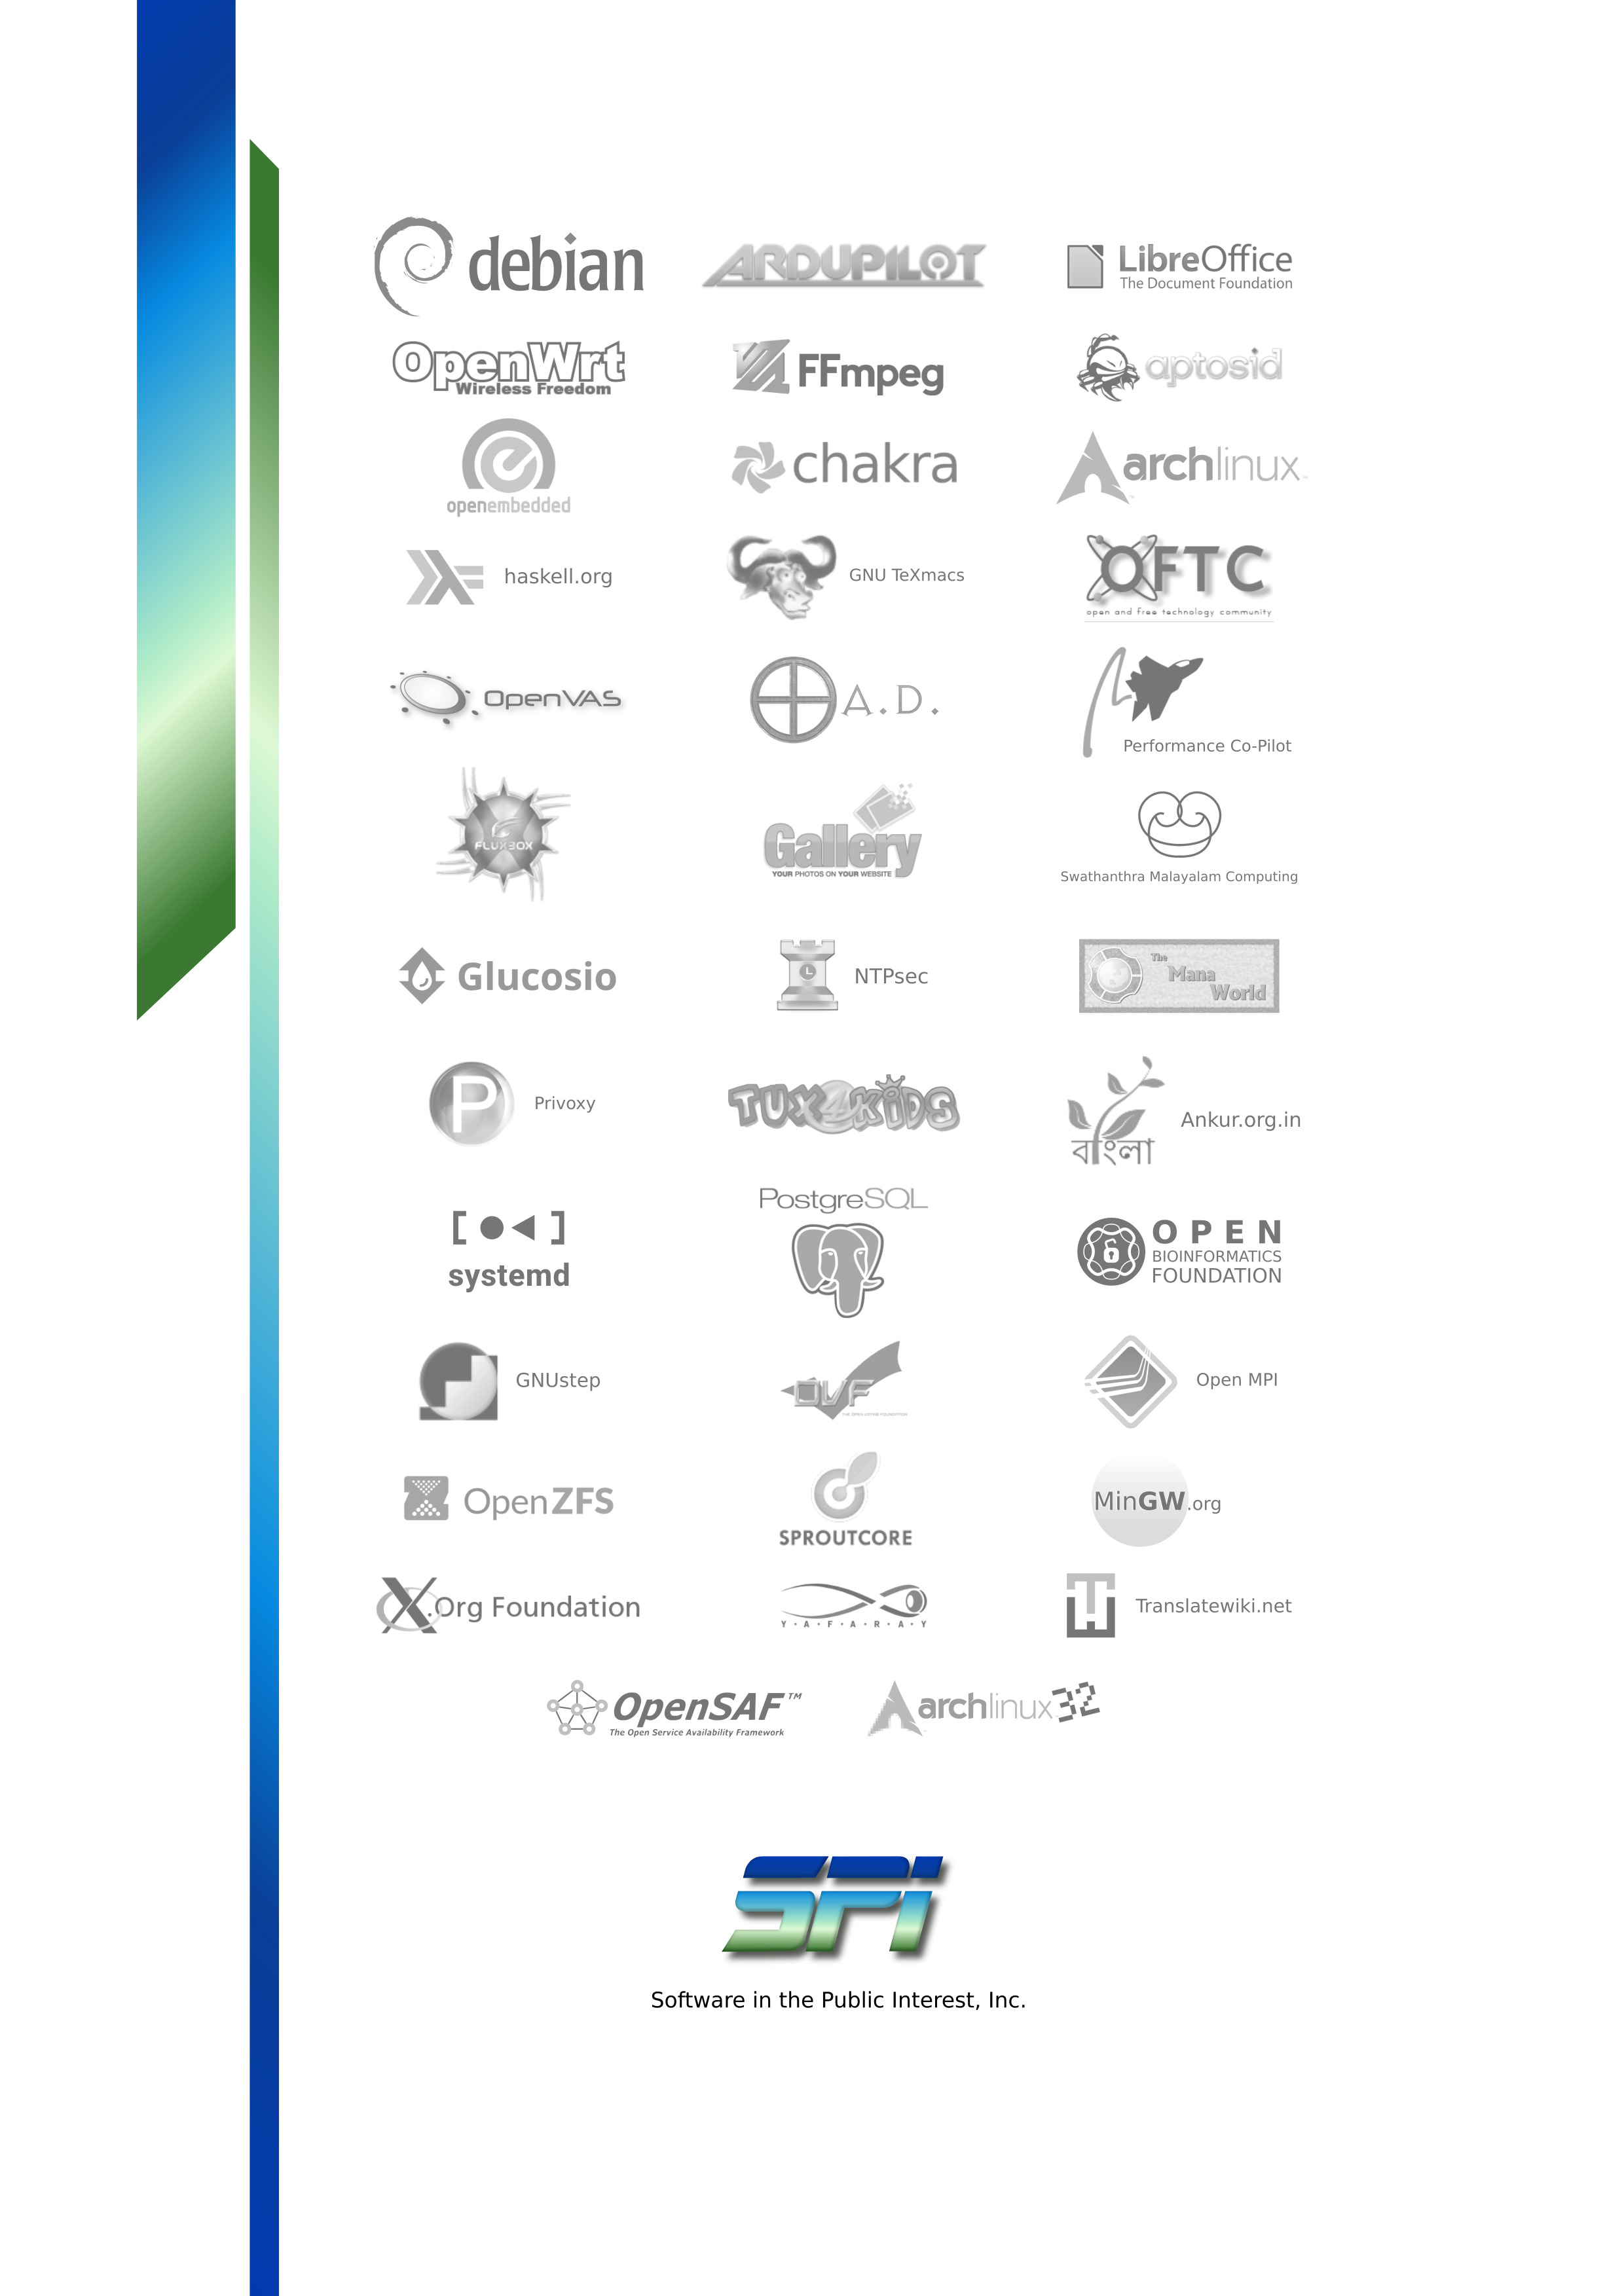
\includegraphics[width=\paperwidth,height=\paperheight]{images/spi-back-2019.jpg}}
}

\null

\end{document}
% Keep this at the bottom, thanks.
% Local Variables:
% TeX-master: "report"
% End:
